\subsection{Grobkonzept 4} \label{subsec:grobkonzept3}
\begin{table}[H]
\footnotesize
\begin{tabular}{>{\HY\RaggedRight}p{3cm} >{\HY\RaggedRight}p{2.2cm} >{\HY\RaggedRight}p{4cm} >{\HY\RaggedRight}p{3.3cm} >{\HY\RaggedRight}p{1.2cm}}
\hline
	\textbf{Bestandteil}		&\textbf{Typ}			&\textbf{Funktion}									&\textbf{Specs}			&\textbf{Anz.}\\
	\hline
\rowcolor{dgelb}
\multicolumn{5}{l}{\textbf{Stromerzeugung}}\\
	Wasserlift 				& 				&Umwandlung in Rotationsenergie						&							&5	\\
	Generator					&Gleichstrom			&Umwandlung in elektrische Energie					&							&5	\\
\rowcolor{dblau}
\multicolumn{5}{l}{\textbf{Elektrotechnik}}\\
 	Wechselrichter				&						&Einspeisung ins Stromnetz							&							&1	\\
 &		& 		&		&\\
\rowcolor{dpink}
\multicolumn{5}{l}{\textbf{Bedienung}}\\
 	Anzeige 					&Display					&zeigt Tankfüllstände und die Generatordaten an 	&							&1	\\
 					&						& 	&							&	\\
\rowcolor{dgruen}
\multicolumn{5}{l}{\textbf{Abwassertechnik}}\\
Bypass						&Absperrklappe						&Umleitung für Wartungsarbeiten am Wasserlift 				&							&	6\\
Leitung	&						&für Wartungsarbeiten 	&							&	1\\
\hline
\end{tabular}
\end{table}
Im Grobkonzepts 4 wird die potenzielle Energie des Wassers mit der Wasserlifttechnik ausgenutzt. Das Abwasser fliesst in eine Schaufel und wird in der Schaufel im Rohr nach unten transportier.So mit erhält der Lift eine Bewegung nach unten und entleer sich am tiefsten Punkt das Abwasser.Somit ist die Leitung nie komplett mit Wasser gefüllt,daher kommt es zu einem Luftwiderstand in den Leitung, der das Abwasser abbremst.
\newpage
\begin{wrapfigure}{r}{0.5\textwidth}
  \begin{center}
    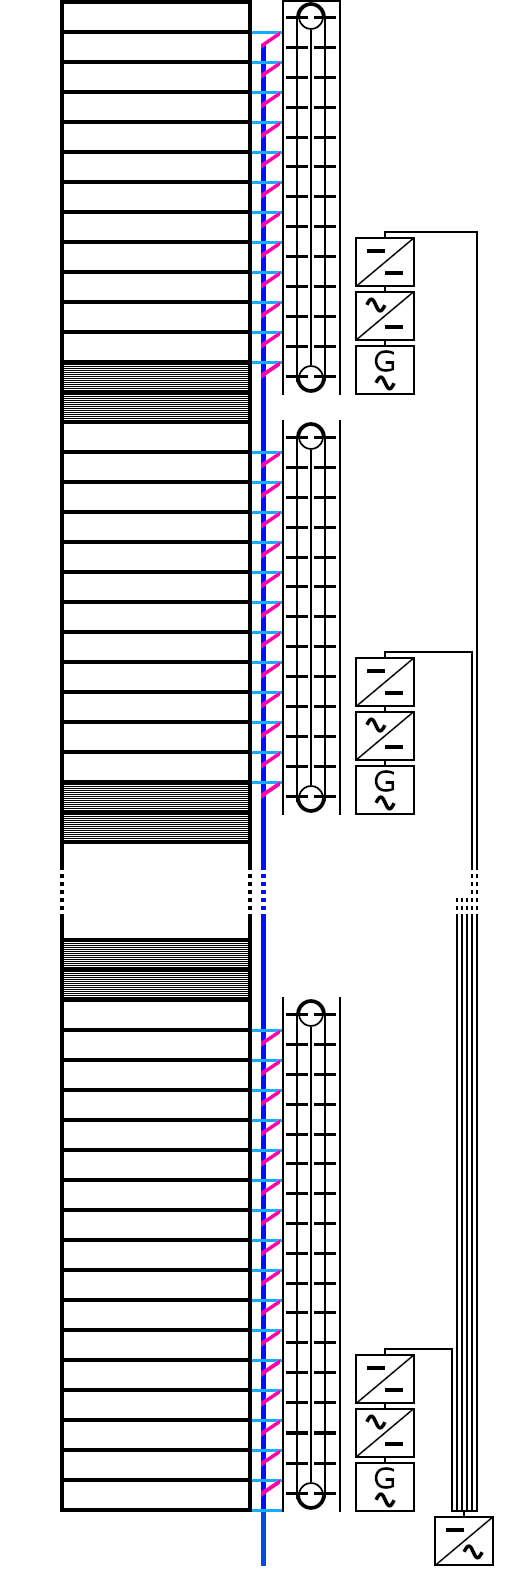
\includegraphics[width=0.48\textwidth]{grobkonzept4}
  \end{center}
  \caption{Grobkonzept 4}
\end{wrapfigure}
Die 5 lifte haben eine Länge von 66.08m und der unterste Lift eine Länge von 80.24m.Für Wartungsarbeiten existiert eine zusätzliche Leitung die mittels Bypass angesteurt wird.

\textbf{Vorteile:}							\newline
+	kostengünstig							\newline
													\newline
\textbf{Nachteile:}\newline
-	defekt anfälliger						\newline
-	umbau										\newline
-	Verstopfungsresistent				\newline	
\WFclear			
\newpage